\pdfoutput=1
\documentclass[11pt]{article}

% ── Packages ──────────────────────────────────────────────────────────
\usepackage[margin=1in]{geometry}
\usepackage{graphicx}
\usepackage{booktabs}
\usepackage{hyperref}
\usepackage{xcolor}
\usepackage{listings}
\usepackage{amsmath}
\usepackage{enumitem}
\usepackage{caption}
\usepackage{subcaption}
\usepackage{url}
\usepackage{tikz}
\usetikzlibrary{shapes.geometric, arrows.meta, positioning, fit, calc}
\usepackage[numbers]{natbib}

\hypersetup{
  colorlinks=true,
  linkcolor=blue!60!black,
  citecolor=green!50!black,
  urlcolor=blue!70!black
}

\lstset{
  basicstyle=\ttfamily\small,
  keywordstyle=\color{blue!70!black}\bfseries,
  commentstyle=\color{green!50!black}\itshape,
  stringstyle=\color{red!60!black},
  breaklines=true,
  frame=single,
  framerule=0.5pt,
  rulecolor=\color{gray!50},
  backgroundcolor=\color{gray!5},
  numbers=left,
  numberstyle=\tiny\color{gray},
  xleftmargin=2em,
  framexleftmargin=1.5em,
  language=Java, % close enough for TypeScript
  morekeywords={async,await,const,let,interface,type,import,export,from,string,number,boolean,void}
}

% ── Title ─────────────────────────────────────────────────────────────
\title{%
  \textbf{Agenti: A Universal Model Context Protocol Server \\
  for Autonomous Blockchain-Enabled AI Agents}
}

\author{
  Nicholas\\
  \texttt{nich.xbt}\\
  \texttt{github.com/nirholas/agenti}
}

\date{March 2026}

% ══════════════════════════════════════════════════════════════════════
\begin{document}
\maketitle

% ── Abstract ──────────────────────────────────────────────────────────
\begin{abstract}
Large language model (LLM) agents are increasingly deployed as autonomous software entities, yet they lack native capabilities for interacting with blockchain infrastructure and making financial transactions. We present \textbf{Agenti}, a universal Model Context Protocol (MCP) server that exposes 380+ blockchain and decentralized finance (DeFi) tools to AI agents across 20+ heterogeneous blockchain networks. Agenti introduces three key contributions: (1)~a multi-chain abstraction layer that unifies EVM, Solana, Cosmos, UTXO, and Move-based chains behind a single tool interface using the CAIP-2 addressing standard; (2)~an integration of the x402 HTTP~402 payment protocol that enables AI agents to autonomously pay for premium services using cryptocurrency with replay-resistant nonce tracking and gasless meta-transactions via EIP-3009; and (3)~a decentralized tool marketplace with smart contract--based registration, DAO-governed dispute resolution, and dynamic pricing models that establishes an economic framework for AI-to-API commerce. We describe the system architecture, security model, and implementation across three MCP transport modes (stdio, HTTP, SSE). Our evaluation demonstrates that Agenti successfully abstracts the complexity of multi-chain interactions while maintaining sub-second tool invocation latency and providing verifiable on-chain payment settlement. Agenti is open-source under the Apache-2.0 license.
\end{abstract}

\noindent\textbf{Keywords:} Model Context Protocol, autonomous agents, blockchain, decentralized finance, x402 payment protocol, multi-chain abstraction, tool marketplace

% ── 1. Introduction ───────────────────────────────────────────────────
\section{Introduction}
\label{sec:introduction}

The emergence of large language models (LLMs) as autonomous software agents~\cite{yao2023react,schick2023toolformer} has created a new class of computing entities that reason, plan, and execute multi-step tasks on behalf of users. Simultaneously, blockchain networks have matured into a diverse ecosystem of over 100 active Layer-1 and Layer-2 chains~\cite{defillama2024}, each offering distinct capabilities in decentralized finance (DeFi), non-fungible tokens (NFTs), governance, and digital payments. The intersection of these two domains---enabling AI agents to interact with blockchain infrastructure autonomously---remains largely unexplored from a systems perspective.

Several challenges impede this integration. First, the \textbf{heterogeneity of blockchain networks} creates a fragmentation problem: EVM-compatible chains, Solana's Sealevel Virtual Machine (SVM), Cosmos's IBC protocol, UTXO-based chains (Bitcoin, Litecoin), and Move-based chains (Sui, Aptos) each require distinct client libraries, transaction formats, and signing mechanisms. An AI agent that must interact with multiple chains today requires bespoke integration code for each. Second, AI agents currently \textbf{lack the ability to make financial transactions}. While humans can approve wallet transactions through browser extensions, autonomous agents require a programmatic payment mechanism with appropriate security guarantees---replay protection, spending limits, and on-chain verifiability. Third, there is \textbf{no economic framework} for AI agents to discover, evaluate, and pay for third-party tools and data services, which limits the composability of agent capabilities.

The Model Context Protocol (MCP)~\cite{anthropic2024mcp} provides a standardized interface for LLM agents to invoke external tools, offering a natural integration point for blockchain capabilities. However, existing MCP servers are either chain-specific or limited to read-only data queries, and none address the payment or marketplace dimensions.

In this paper, we present \textbf{Agenti}, a universal MCP server that addresses these challenges through three contributions:

\begin{enumerate}[leftmargin=*]
  \item \textbf{Multi-Chain Abstraction Layer.} A unified tool interface spanning 20+ blockchain networks (13 EVM chains, Solana, Cosmos, Bitcoin, Litecoin, Dogecoin, Sui, Aptos, Near, TON, XRP) using the CAIP-2~\cite{caip2} chain identification standard. Agenti provides 380+ tools organized into 22 functional modules, accessible through a single MCP server instance.

  \item \textbf{Autonomous Agent Payment Protocol.} An integration of the x402 HTTP~402 payment standard~\cite{coinbase2024x402} that enables AI agents to make cryptocurrency payments without human intervention. Our implementation includes deterministic nonce generation via Keccak-256 hashing, 24-hour time-windowed replay protection, EIP-3009~\cite{eip3009} gasless meta-transactions for USDC, and facilitator signature verification for trusted intermediaries.

  \item \textbf{Decentralized Tool Marketplace.} A smart contract--based marketplace for tool registration, discovery, and monetization, featuring a reputation system (0--100 score), four pricing models (per-call, subscription, tiered, freemium), automated revenue distribution via a \texttt{RevenueRouter} contract, and DAO-governed dispute arbitration.
\end{enumerate}

Agenti is implemented in TypeScript (172,806 lines across 547 files), supports three MCP transport modes, and is deployed as an open-source project under the Apache-2.0 license.

The remainder of this paper is organized as follows. Section~\ref{sec:background} provides necessary background on MCP, blockchain ecosystems, and agent payment protocols. Section~\ref{sec:architecture} describes Agenti's system architecture. Section~\ref{sec:payment} details the x402 payment integration. Section~\ref{sec:marketplace} presents the decentralized tool marketplace. Section~\ref{sec:implementation} covers implementation details. Section~\ref{sec:evaluation} evaluates the system. Section~\ref{sec:related} discusses related work. Section~\ref{sec:conclusion} concludes.

% ── 2. Background ─────────────────────────────────────────────────────
\section{Background and Motivation}
\label{sec:background}

\subsection{Model Context Protocol (MCP)}

The Model Context Protocol~\cite{anthropic2024mcp} is an open standard that defines a JSON-RPC--based interface between LLM applications (clients) and external capability providers (servers). An MCP server exposes \emph{tools}---typed functions with Zod-validated input schemas and structured return values---that an LLM agent can discover and invoke at inference time. MCP supports three transport modes: \textbf{stdio} (standard input/output for local process communication), \textbf{HTTP} (stateful sessions via Streamable HTTP with JSON-RPC), and \textbf{SSE} (Server-Sent Events for legacy web integrations).

The protocol's tool abstraction is well-suited for blockchain interactions because it enforces input validation (preventing malformed transactions), supports structured error responses, and allows the LLM to reason about tool capabilities through natural-language descriptions. However, the protocol itself is agnostic to payment semantics, leaving a gap that Agenti fills.

\subsection{Blockchain Network Heterogeneity}

Modern blockchain ecosystems exhibit significant architectural diversity:

\begin{itemize}[leftmargin=*]
  \item \textbf{EVM chains} (Ethereum, Arbitrum, Base, Polygon, etc.) share a common execution environment but differ in gas mechanics (EIP-1559 vs. legacy), L2 data availability strategies, and RPC endpoint behavior.
  \item \textbf{SVM chains} (Solana) use a fundamentally different account model, transaction format (versioned messages), and signing scheme (Ed25519 vs. ECDSA).
  \item \textbf{UTXO chains} (Bitcoin, Litecoin, Dogecoin) use unspent transaction outputs rather than account balances, requiring distinct transaction construction.
  \item \textbf{Cosmos/IBC chains} use Tendermint consensus with inter-blockchain communication for cross-chain messaging.
  \item \textbf{Move-based chains} (Sui, Aptos) use an object-centric model with the Move programming language.
\end{itemize}

An AI agent interacting with this ecosystem must handle chain-specific client instantiation, transaction signing, fee estimation, and confirmation tracking---complexity that Agenti abstracts behind a uniform tool interface.

\subsection{The HTTP 402 Payment Required Status Code}

HTTP~402 was reserved in RFC~7231~\cite{rfc7231} for ``future use'' as a payment-required response code. The x402 protocol~\cite{coinbase2024x402} operationalizes this code for machine-to-machine cryptocurrency payments. When a server returns HTTP~402, the response includes payment requirements (amount, token, recipient address, chain). A compliant client constructs and submits a blockchain transaction, then retries the original request with a payment proof header (\texttt{x-payment-proof}). This creates a stateless, RESTful payment flow suitable for autonomous agents.

\subsection{Motivating Scenario}

Consider an AI agent tasked with portfolio rebalancing across multiple chains. The agent must: (1)~query token balances on Ethereum, Arbitrum, and Solana; (2)~fetch real-time prices from CoinGecko; (3)~compute optimal allocation; (4)~execute swaps via DEX aggregators (1inch, Jupiter); (5)~bridge assets cross-chain via LayerZero; and (6)~pay for premium analytics data using x402. Without Agenti, this requires integrating 6+ distinct SDKs, managing 3+ signing mechanisms, and implementing custom payment logic. With Agenti, each step is a single MCP tool call against a unified interface.

% ── 3. System Architecture ────────────────────────────────────────────
\section{System Architecture}
\label{sec:architecture}

Agenti is structured as a layered system with four principal components: the \emph{transport layer}, the \emph{tool registry}, the \emph{chain abstraction layer}, and the \emph{payment subsystem}. Figure~\ref{fig:architecture} illustrates the high-level architecture.

\begin{figure}[t]
\centering
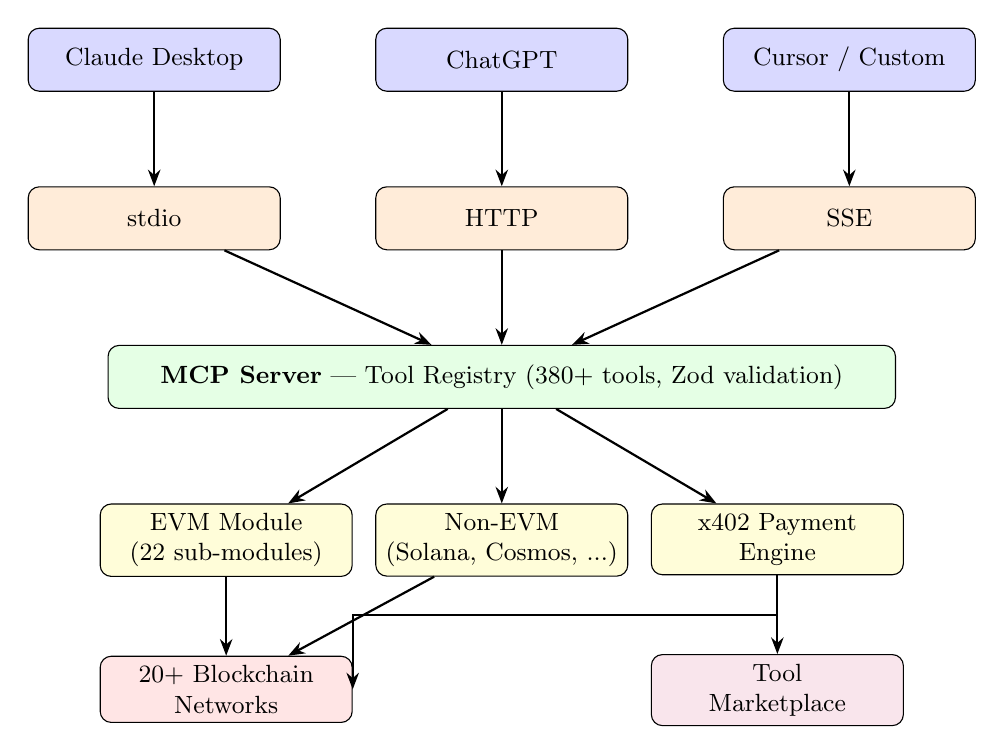
\begin{tikzpicture}[
  node distance=0.8cm and 1.2cm,
  box/.style={draw, rounded corners, minimum width=3.2cm, minimum height=0.8cm, align=center, font=\small},
  bigbox/.style={draw, rounded corners, minimum width=10cm, minimum height=0.8cm, align=center, font=\small},
  layer/.style={draw, dashed, rounded corners, inner sep=8pt, fill=#1!5},
  arrow/.style={-{Stealth[length=6pt]}, thick},
]

% Agents
\node[box, fill=blue!15] (claude) {Claude Desktop};
\node[box, fill=blue!15, right=of claude] (chatgpt) {ChatGPT};
\node[box, fill=blue!15, right=of chatgpt] (cursor) {Cursor / Custom};

% Transport
\node[box, fill=orange!15, below=1.2cm of claude] (stdio) {stdio};
\node[box, fill=orange!15, below=1.2cm of chatgpt] (http) {HTTP};
\node[box, fill=orange!15, below=1.2cm of cursor] (sse) {SSE};

% MCP Server
\node[bigbox, fill=green!10, below=1.2cm of http] (mcp) {\textbf{MCP Server} --- Tool Registry (380+ tools, Zod validation)};

% Lower modules
\node[box, fill=yellow!15, below=1.2cm of mcp, xshift=-3.5cm] (evm) {EVM Module\\(22 sub-modules)};
\node[box, fill=yellow!15, below=1.2cm of mcp] (nonev) {Non-EVM\\(Solana, Cosmos, ...)};
\node[box, fill=yellow!15, below=1.2cm of mcp, xshift=3.5cm] (x402) {x402 Payment\\Engine};

% Chains
\node[box, fill=red!10, below=1cm of evm] (chains) {20+ Blockchain\\Networks};
\node[box, fill=purple!10, below=1cm of x402] (market) {Tool\\Marketplace};

% Arrows
\draw[arrow] (claude) -- (stdio);
\draw[arrow] (chatgpt) -- (http);
\draw[arrow] (cursor) -- (sse);
\draw[arrow] (stdio) -- (mcp);
\draw[arrow] (http) -- (mcp);
\draw[arrow] (sse) -- (mcp);
\draw[arrow] (mcp) -- (evm);
\draw[arrow] (mcp) -- (nonev);
\draw[arrow] (mcp) -- (x402);
\draw[arrow] (evm) -- (chains);
\draw[arrow] (nonev) -- (chains);
\draw[arrow] (x402) -- (market);
\draw[arrow] (x402.south) -- ++(0,-0.5) -| (chains.east);

\end{tikzpicture}
\caption{Agenti system architecture. AI agents connect via one of three MCP transport modes. The tool registry dispatches requests to chain-specific modules or the x402 payment engine. All chain interactions flow through the multi-chain abstraction layer.}
\label{fig:architecture}
\end{figure}

\subsection{Transport Layer}

Agenti supports three MCP transport modes, each serving different deployment contexts:

\paragraph{Standard I/O (stdio).} The default transport for local integrations (e.g., Claude Desktop). Bidirectional JSON-RPC messages are exchanged over stdin/stdout, with error logging on stderr. This mode has zero network overhead and is suitable for single-agent deployments.

\paragraph{Streamable HTTP.} The modern transport for web-based agents (e.g., ChatGPT Developer Mode). Agenti implements stateful session management using UUID-based session identifiers transmitted via the \texttt{mcp-session-id} header. The server exposes three endpoints: \texttt{POST /mcp} for JSON-RPC requests, \texttt{GET /mcp} for server-initiated SSE notifications, and \texttt{DELETE /mcp} for session termination. CORS headers expose \texttt{mcp-session-id} and \texttt{x-payment-proof} for cross-origin agent access.

\paragraph{Server-Sent Events (SSE).} A legacy transport maintained for backward compatibility. Multi-session support is implemented via a session ID mapping, with \texttt{GET /sse} initiating connections and \texttt{POST /messages?sessionId=\{id\}} handling requests.

\subsection{Tool Registry}

Tools are the fundamental unit of functionality in Agenti. Each tool is defined by a name, natural-language description, a Zod input schema, and an asynchronous execution function. The registry pattern follows a composable registration approach:

\begin{lstlisting}[caption={Tool registration pattern in Agenti.},label={lst:toolreg}]
server.tool(
  "get_token_balance",
  "Get the balance of an ERC-20 token for an address",
  {
    chainId: z.number().describe("EVM chain ID"),
    address: z.string().describe("Wallet address"),
    tokenAddress: z.string().describe("Token contract")
  },
  async (params) => {
    const validated = inputSchema.parse(params);
    const balance = await getBalance(validated);
    return {
      content: [{ type: "text", text: JSON.stringify(balance) }]
    };
  }
);
\end{lstlisting}

At startup, the server composes modules via functional registration:

\begin{lstlisting}[caption={Module composition at server initialization.},label={lst:compose}]
const server = new McpServer({
  name: "Universal Crypto MCP",
  version: "1.1.0"
});
registerEVM(server);          // 22 sub-modules
registerX402(server);         // Payment tools
registerToolMarketplace(server);
registerVendors(server);      // 25 integrations
\end{lstlisting}

This composition yields 380+ tools organized into the categories shown in Table~\ref{tab:tools}.

\begin{table}[t]
\centering
\caption{Tool categories and representative capabilities in Agenti.}
\label{tab:tools}
\begin{tabular}{@{}llr@{}}
\toprule
\textbf{Category} & \textbf{Representative Tools} & \textbf{Count} \\
\midrule
Network \& Blocks     & Chain info, gas prices, block retrieval       & 18 \\
Transactions          & Submit, trace, receipt, status                 & 22 \\
Tokens \& NFTs        & ERC-20/721/1155 ops, metadata                 & 35 \\
Wallet \& Portfolio   & Balances, transfers, position tracking         & 28 \\
DeFi --- Swap         & 1inch, 0x, ParaSwap, Jupiter aggregation      & 24 \\
DeFi --- Lending      & Aave, Compound supply/borrow                  & 16 \\
DeFi --- Staking      & Lido, native staking, yield calc              & 12 \\
Bridge                & LayerZero, Stargate, Wormhole                 & 18 \\
Security              & Honeypot, rug pull, GoPlus, approvals         & 22 \\
Market Data           & CoinGecko, DefiLlama, fear/greed              & 30 \\
Technical Analysis    & 50+ indicators (RSI, MACD, Bollinger)         & 52 \\
Governance            & Snapshot, on-chain proposals, voting           & 14 \\
MEV \& Gas            & Flashbots, gas optimization, EIP-1559         & 10 \\
x402 Payments         & Pay, verify, balance, yield, gasless           & 14 \\
DEX Analytics         & GeckoTerminal, DexPaprika, whale tracking     & 26 \\
Domains               & ENS resolution, reverse lookup                & 8  \\
Contract Interaction  & ABI parsing, read/write, deployment           & 20 \\
Signatures            & EIP-712, message signing, verification        & 8  \\
Marketplace           & Register, discover, rate, stake                & 12 \\
\midrule
\textbf{Total}        &                                               & \textbf{389} \\
\bottomrule
\end{tabular}
\end{table}

\subsection{Multi-Chain Abstraction Layer}
\label{sec:multichain}

The chain abstraction layer provides a uniform interface across heterogeneous blockchain architectures. The key design decisions are:

\paragraph{CAIP-2 Chain Identification.} All chains are identified using the Chain Agnostic Improvement Proposal 2 (CAIP-2) standard~\cite{caip2}, which encodes chains as \texttt{namespace:reference} pairs. For example, Ethereum mainnet is \texttt{eip155:1}, Base is \texttt{eip155:8453}, and Solana mainnet is \texttt{solana:5eykt4UsFv8P8NJdTREpY1vzqKqZKvdp} (using the cluster genesis hash). This enables unambiguous chain references across the entire tool surface.

\paragraph{Client Factory Pattern.} Agenti uses \texttt{viem}~\cite{viem} as the primary EVM client library, instantiating public and wallet clients per-chain via a factory pattern:

\begin{lstlisting}[caption={Chain-specific client instantiation.},label={lst:client}]
const client = createPublicClient({
  chain: resolveViemChain(chainId),
  transport: http(getRpcUrl(chainId))
});
\end{lstlisting}

For non-EVM chains, dedicated client libraries are used: \texttt{@solana/web3.js} for Solana, \texttt{xchainjs} for UTXO chains, \texttt{@cosmjs} for Cosmos/IBC, and chain-specific SDKs for Sui, Aptos, Near, and TON.

\paragraph{Adaptive Transaction Construction.} Each chain family requires distinct transaction construction logic:
\begin{itemize}[leftmargin=*]
  \item \textbf{EVM}: EIP-1559 fee estimation with legacy fallback, nonce management via \texttt{getTransactionCount}, gas limit estimation.
  \item \textbf{SVM}: Versioned messages with recent blockhash, compute unit pricing, priority fee estimation via \texttt{getRecentPrioritizationFees}.
  \item \textbf{UTXO}: Input selection (coin control), change address derivation, fee-rate estimation via \texttt{estimateSmartFee}.
  \item \textbf{Cosmos}: Amino/Protobuf message encoding, gas simulation via \texttt{simulate}, IBC channel resolution for cross-chain transfers.
\end{itemize}

\paragraph{DEX Aggregation with Fallback.} For swap operations, Agenti implements a three-tier aggregation strategy: 1inch $\rightarrow$ 0x $\rightarrow$ ParaSwap, where each aggregator is attempted in order. On Solana, Jupiter serves as the primary aggregator. This ensures maximum liquidity access while providing resilience against individual aggregator downtime.

% ── 4. x402 Payment Protocol ─────────────────────────────────────────
\section{Autonomous Agent Payments via x402}
\label{sec:payment}

A defining capability of Agenti is enabling AI agents to make cryptocurrency payments autonomously. This section describes the x402 integration in detail.

\subsection{Protocol Overview}

The x402 payment flow operates as follows:

\begin{enumerate}[leftmargin=*]
  \item An AI agent invokes a tool that requires payment (e.g., premium analytics data).
  \item The service returns HTTP~402 with payment requirements: amount, token address (USDC), recipient, chain ID, and a payment nonce.
  \item Agenti's payment engine constructs a blockchain transaction (or EIP-3009 authorization for gasless transfers), signs it with the agent's private key, and submits it to the network.
  \item Upon transaction confirmation, Agenti constructs a payment proof containing the transaction hash, block number, and nonce.
  \item The original request is retried with the \texttt{x-payment-proof} header, and the service verifies the proof on-chain before responding.
\end{enumerate}

\subsection{Supported Chains and Tokens}

Agenti supports x402 payments on six EVM chains (Ethereum, Arbitrum, Base, Polygon, Optimism, BSC) and Solana, with corresponding testnets. The primary payment token is USDC (6 decimals), with additional support for USDs (Sperax USD, 18 decimals), USDT, and DAI. Token addresses are maintained in a chain-indexed registry with checksum validation.

\subsection{Replay Protection via Nonce Tracking}
\label{sec:nonce}

Replay attacks are the primary security concern in automated payment systems. Agenti implements a multi-layered nonce tracking system:

\paragraph{Deterministic Payment ID.} Each payment is assigned a unique identifier via Keccak-256 hashing:

$$\text{paymentId} = \text{keccak256}(\texttt{chainId} \| \texttt{:} \| \texttt{txHash} \| \texttt{:} \| \texttt{logIndex})[0{:}18]$$

This deterministic construction ensures that the same on-chain event always maps to the same payment ID, preventing double-crediting across server restarts.

\paragraph{In-Memory Nonce Store.} Used nonces are tracked in a bounded map with the following invariants:
\begin{itemize}[leftmargin=*]
  \item \textbf{Capacity}: Maximum 100,000 concurrent entries, with LRU eviction when full.
  \item \textbf{TTL}: 24-hour expiry per nonce, enforced via periodic cleanup.
  \item \textbf{Atomicity}: \texttt{isNonceUsed()} and \texttt{markNonceUsed()} are executed sequentially to prevent TOCTOU races in single-threaded Node.js execution.
\end{itemize}

\paragraph{Security Event Logging.} Replay attempts trigger critical-level security events, enabling monitoring and alerting in production deployments.

\subsection{Gasless Transfers via EIP-3009}
\label{sec:gasless}

A significant barrier to AI agent payments is the requirement to hold native tokens (ETH, SOL) for gas fees. Agenti leverages EIP-3009~\cite{eip3009} (Transfer With Authorization), supported by USDC on major EVM chains, to enable gasless transfers:

\begin{enumerate}[leftmargin=*]
  \item The agent signs an off-chain authorization specifying \texttt{from}, \texttt{to}, \texttt{value}, \texttt{validAfter}, \texttt{validBefore}, and a unique \texttt{nonce}.
  \item Any relayer (including the payment recipient) can submit the authorization on-chain, paying gas on behalf of the agent.
  \item The USDC contract verifies the ECDSA signature and executes the transfer.
\end{enumerate}

This mechanism allows an agent wallet funded solely with USDC to make payments without requiring ETH for gas, significantly simplifying wallet management.

\subsection{Facilitator Verification}

For trusted intermediary scenarios, Agenti supports optional facilitator signatures on payment proofs. The verification uses EIP-191 message recovery:

$$\text{signer} = \texttt{recoverMessageAddress}(\text{proofMessage}, \text{signature})$$

The recovered signer is checked against a registry of trusted facilitators. This enables payment aggregation services where a facilitator batches multiple agent payments into a single on-chain transaction.

\subsection{Payment Proof Structure}

\begin{lstlisting}[caption={Payment proof data structure.},label={lst:proof}]
interface PaymentProof {
  txHash: string;          // Transaction hash
  chainId: number;         // Chain identifier
  from: Address;           // Payer (agent wallet)
  to: Address;             // Recipient (service)
  amount: string;          // Token amount (smallest unit)
  token: Address;          // Token contract address
  blockNumber: number;     // Confirmation block
  timestamp: number;       // Block timestamp
  nonce: string;           // Unique payment nonce
  facilitatorSignature?: string;
}
\end{lstlisting}

Verification follows five steps: (1)~nonce uniqueness check, (2)~recipient validation, (3)~amount validation, (4)~facilitator signature verification (if present), and (5)~nonce marking.

% ── 5. Decentralized Tool Marketplace ─────────────────────────────────
\section{Decentralized Tool Marketplace}
\label{sec:marketplace}

Agenti includes a decentralized marketplace that enables third-party developers to publish, monetize, and govern MCP tools via smart contracts.

\subsection{Smart Contract Architecture}

The marketplace is implemented across four smart contracts deployed on Arbitrum, Base, and Optimism (with testnet counterparts):

\begin{itemize}[leftmargin=*]
  \item \textbf{ToolRegistry}: Stores tool metadata (name, description, version, author, endpoint), handles registration and version updates. Each tool is identified by a unique \texttt{toolId}.
  \item \textbf{RevenueRouter}: Routes payment flows from tool consumers to creators. Supports configurable revenue splits (default: 80\% creator, 15\% platform, 5\% fee). Minimum payout threshold: \$1.00.
  \item \textbf{ToolStaking}: Enables tool developers to stake tokens as a quality signal. Staked tools receive higher visibility in discovery and are eligible for dispute arbitration coverage.
  \item \textbf{ArbitrationDAO}: Governs dispute resolution for quality complaints, refund requests, and tool de-listing. Decisions are made via weighted voting proportional to stake.
\end{itemize}

\subsection{Pricing Models}

The marketplace supports four pricing models to accommodate diverse tool economics:

\begin{table}[h]
\centering
\caption{Marketplace pricing models.}
\label{tab:pricing}
\begin{tabular}{@{}lll@{}}
\toprule
\textbf{Model} & \textbf{Mechanism} & \textbf{Use Case} \\
\midrule
Per-Call    & Fixed price per invocation (\$0.001--\$10)   & Premium API endpoints \\
Subscription & Monthly recurring with call limits          & High-frequency analytics \\
Tiered      & Volume discounts at usage thresholds         & Growing agent teams \\
Freemium    & Free daily quota + paid overage              & Developer onboarding \\
\bottomrule
\end{tabular}
\end{table}

\subsection{Reputation System}

Tool quality is tracked via a reputation score ranging from 0 to 100, computed as a weighted combination of:

\begin{equation}
\text{score} = 0.4 \cdot \bar{r} \cdot 20 + 0.25 \cdot u + 0.2 \cdot (1 - \bar{t}/t_{\max}) \cdot 100 + 0.15 \cdot h
\label{eq:reputation}
\end{equation}

where $\bar{r}$ is the mean user rating (1--5 stars), $u$ is uptime percentage, $\bar{t}$ is average response time, $t_{\max}$ is the maximum acceptable response time, and $h$ is a historical reliability score based on incident frequency.

\subsection{Revenue Distribution}

Revenue distribution occurs via the \texttt{RevenueRouter} contract. When a tool invocation generates revenue, the router:
\begin{enumerate}[leftmargin=*]
  \item Records the payment against the tool's \texttt{toolId}.
  \item Applies the configured revenue split (stored as \texttt{RevenueSplit[]} with address and percentage).
  \item Accumulates payments until the payout threshold (\$1.00) is reached.
  \item Executes batch transfers in USDs or USDC to all split recipients.
\end{enumerate}

This on-chain revenue model creates transparent, verifiable compensation for tool developers---a property absent from centralized tool platforms.

% ── 6. Implementation ─────────────────────────────────────────────────
\section{Implementation}
\label{sec:implementation}

\subsection{Technology Stack}

Agenti is implemented in TypeScript under strict mode, comprising 172,806 lines of code across 547 files. Table~\ref{tab:deps} summarizes the key dependencies.

\begin{table}[h]
\centering
\caption{Key dependencies and their roles.}
\label{tab:deps}
\begin{tabular}{@{}lll@{}}
\toprule
\textbf{Dependency} & \textbf{Version} & \textbf{Role} \\
\midrule
\texttt{@modelcontextprotocol/sdk} & 1.26.0 & MCP protocol implementation \\
\texttt{viem}                       & 2.46.2 & EVM client library \\
\texttt{zod}                        & 4.3.6  & Runtime input validation \\
\texttt{@x402/core}                 & 2.3.0  & x402 payment protocol \\
\texttt{@x402/evm}                  & 2.3.1  & EVM payment mechanism \\
\texttt{@x402/svm}                  & 2.4.0  & Solana payment mechanism \\
\texttt{@solana/web3.js}            & 1.87.6 & Solana client \\
\texttt{ccxt}                       & 4.5.36 & Exchange data (400+ exchanges) \\
\texttt{express}                    & 4.22.1 & HTTP server framework \\
\bottomrule
\end{tabular}
\end{table}

\subsection{Build and Deployment}

The project uses \texttt{tsup} for bundling, producing both ESM and CommonJS outputs with TypeScript definition files. The build pipeline runs in under 30 seconds. Deployment options include:

\begin{itemize}[leftmargin=*]
  \item \textbf{Local}: \texttt{npm start} launches the stdio server for Claude Desktop integration.
  \item \textbf{HTTP server}: \texttt{npm run start:http} for web-based agent access.
  \item \textbf{Docker}: Multi-stage Dockerfile with a 150MB production image.
\end{itemize}

\subsection{Testing Infrastructure}

Agenti employs a three-tier testing strategy:

\begin{itemize}[leftmargin=*]
  \item \textbf{Unit tests}: Co-located with source files (\texttt{*.test.ts}), using Vitest with custom matchers (\texttt{toBeSuccessfulToolResponse}, \texttt{toContainValidAddress}, \texttt{toContainValidTxHash}).
  \item \textbf{Integration tests}: Multi-component tests with mocked blockchain clients (viem public/wallet clients return predictable data) and HTTP interceptors.
  \item \textbf{End-to-end tests}: Full server startup against stdio transport, exercising the complete MCP request/response lifecycle.
\end{itemize}

The test suite comprises 1,945 test cases with coverage thresholds of 80\% for statements, functions, and lines, and 75\% for branches.

\subsection{Security Considerations}

\paragraph{Private Key Management.} Agent private keys are loaded exclusively from environment variables (\texttt{X402\_PRIVATE\_KEY}, \texttt{PRIVATE\_KEY}), never committed to source control. Keys are validated for format correctness (hex with \texttt{0x} prefix for EVM, Base58 for Solana) at startup.

\paragraph{Mainnet Protection.} Mainnet operations require explicit opt-in via \texttt{X402\_MAINNET\_ENABLED=true}. The default configuration targets testnets (Sepolia, Base Sepolia), preventing accidental mainnet transactions during development.

\paragraph{Input Validation.} All tool inputs are validated through Zod schemas before execution. Address inputs undergo EIP-55 checksum validation, URLs are checked against RFC~3986, and chain IDs are verified against the supported chain registry.

\paragraph{Security Scanning.} Agenti integrates GoPlus security APIs for runtime safety checks: token contract analysis (honeypot detection, mint function presence, pause mechanisms), dApp phishing detection, and address risk scoring.

% ── 7. Evaluation ─────────────────────────────────────────────────────
\section{Evaluation}
\label{sec:evaluation}

We evaluate Agenti along four dimensions: tool coverage, multi-chain abstraction effectiveness, payment protocol performance, and developer experience.

\subsection{Tool Coverage Comparison}

Table~\ref{tab:comparison} compares Agenti with existing blockchain tooling approaches available to AI agents.

\begin{table}[h]
\centering
\caption{Comparison with existing blockchain tooling for AI agents.}
\label{tab:comparison}
\begin{tabular}{@{}lccccc@{}}
\toprule
\textbf{System} & \textbf{Tools} & \textbf{Chains} & \textbf{MCP} & \textbf{Payments} & \textbf{Marketplace} \\
\midrule
Direct RPC           & --- & 1     & No  & No  & No  \\
Ethers.js / web3.js  & --- & EVM   & No  & No  & No  \\
Chain-specific MCP   & 10--50 & 1  & Yes & No  & No  \\
LangChain Web3       & 20--30 & EVM & No  & No  & No  \\
\textbf{Agenti}      & \textbf{389} & \textbf{20+} & \textbf{Yes} & \textbf{Yes} & \textbf{Yes} \\
\bottomrule
\end{tabular}
\end{table}

Agenti provides an order-of-magnitude improvement in tool coverage while being the only system to support autonomous payments and a decentralized marketplace.

\subsection{Multi-Chain Abstraction}

To evaluate the abstraction layer's effectiveness, we measure the developer effort required to add support for a new chain. Adding a new EVM chain requires:
\begin{enumerate}[leftmargin=*]
  \item Adding the chain configuration to the chain registry (chain ID, RPC URL, explorer URL): \textbf{5 lines of code}.
  \item If the chain is supported by \texttt{viem}, no additional client code is needed.
  \item All 22 EVM modules automatically apply to the new chain.
\end{enumerate}

For non-EVM chains, the effort is higher but bounded: Solana integration required approximately 2,000 lines; Cosmos/IBC required approximately 1,500 lines. In both cases, the tools are immediately accessible via the MCP interface without changes to the transport layer.

\subsection{Payment Protocol Characteristics}

The x402 payment subsystem exhibits the following characteristics:
\begin{itemize}[leftmargin=*]
  \item \textbf{Nonce capacity}: 100,000 concurrent nonces with LRU eviction, supporting high-throughput agent deployments.
  \item \textbf{Replay window}: 24-hour TTL provides sufficient protection while bounding memory usage.
  \item \textbf{Settlement finality}: Depends on the underlying chain---approximately 12 seconds on Ethereum L1, sub-second on L2s (Arbitrum, Base), and 400ms on Solana.
  \item \textbf{Gasless transfer support}: EIP-3009 eliminates the need for agents to hold native tokens, reducing wallet management complexity from two tokens (USDC + ETH) to one (USDC).
\end{itemize}

\subsection{Developer Experience}

We assess developer experience through the integration workflow. Connecting an AI agent (Claude Desktop) to Agenti requires a single configuration entry:

\begin{lstlisting}[language={}]
{
  "mcpServers": {
    "agenti": {
      "command": "npx",
      "args": ["@nirholas/agenti"]
    }
  }
}
\end{lstlisting}

Once connected, the agent can invoke any of the 389 tools via natural language, with Zod schemas providing automatic parameter validation and descriptive error messages. No blockchain-specific knowledge is required on the agent side.

% ── 8. Related Work ───────────────────────────────────────────────────
\section{Related Work}
\label{sec:related}

\paragraph{AI Agent Frameworks.} ReAct~\cite{yao2023react} and Toolformer~\cite{schick2023toolformer} establish the paradigm of LLMs as tool-using agents. LangChain~\cite{langchain} and AutoGPT~\cite{autogpt} provide general-purpose agent frameworks with limited blockchain support. Agenti complements these frameworks by providing the blockchain-specific tool layer accessible via MCP.

\paragraph{Blockchain Developer Tools.} Ethers.js~\cite{ethersjs}, web3.js~\cite{web3js}, and viem~\cite{viem} provide programmatic access to EVM chains but require manual integration per chain and are not designed for LLM consumption. Hardhat~\cite{hardhat} and Foundry~\cite{foundry} focus on smart contract development rather than agent interaction. Agenti builds on viem to provide an LLM-native interface.

\paragraph{MCP Servers for Web3.} Several chain-specific MCP servers exist (e.g., for Ethereum, Solana), typically providing 10--50 tools for a single chain. Agenti differs in its universal multi-chain support, payment integration, and marketplace economics.

\paragraph{Machine-to-Machine Payments.} The Lightning Network~\cite{poon2016lightning} enables fast Bitcoin micropayments but requires channel management. Raiden Network~\cite{raiden} brings payment channels to Ethereum. The x402 protocol~\cite{coinbase2024x402} provides a simpler, RESTful payment model suitable for AI agents. Agenti is the first system to integrate x402 into an MCP server context.

\paragraph{Decentralized Marketplaces.} Ocean Protocol~\cite{ocean} provides a marketplace for data assets. SingularityNET~\cite{singularitynet} offers an AI service marketplace. Agenti's tool marketplace is distinct in its MCP-native design, Zod-validated tool schemas, and integration with the x402 payment layer.

% ── 9. Discussion ─────────────────────────────────────────────────────
\section{Discussion}
\label{sec:discussion}

\paragraph{Limitations.} Agenti's nonce store is in-memory, which means nonces are lost on server restart. A persistent store (e.g., Redis, SQLite) would be required for production deployments with strict replay guarantees. The tool marketplace smart contracts are deployed on L2 chains for cost efficiency, but this introduces bridge latency for cross-chain tool payments. The system currently relies on a single maintainer, which affects the pace of chain additions and vulnerability response.

\paragraph{Trust Model.} Agenti trusts the MCP client (AI agent) to act within its configured spending limits. The private key held by the agent wallet is the root of trust---compromising it enables unauthorized payments. Future work should explore multi-signature wallets, spending caps enforced at the smart contract level, and hardware security module (HSM) integration for high-value deployments.

\paragraph{Scalability.} The current architecture supports a single server instance per agent. Scaling to multi-agent deployments requires session isolation (provided by the HTTP transport's UUID-based sessions) and shared nonce stores. Horizontal scaling behind a load balancer is straightforward given the stateless tool execution model, though session affinity is required for the SSE transport.

\paragraph{Ethical Considerations.} Autonomous agent payments raise questions about accountability---if an agent makes an erroneous payment, liability is unclear. Agenti mitigates this through spending limits, testnet defaults, and explicit mainnet opt-in, but broader regulatory and ethical frameworks are needed as agent payment capabilities mature.

% ── 10. Conclusion ────────────────────────────────────────────────────
\section{Conclusion}
\label{sec:conclusion}

We have presented Agenti, a universal MCP server that bridges the gap between AI agents and blockchain infrastructure. By unifying 380+ tools across 20+ heterogeneous chains behind a single protocol interface, integrating autonomous cryptocurrency payments via x402, and establishing a decentralized tool marketplace with DAO governance, Agenti provides the systems infrastructure necessary for AI agents to operate as autonomous economic entities in the blockchain ecosystem.

Our key insight is that the Model Context Protocol's tool abstraction is a natural fit for blockchain interactions---it provides the input validation, structured responses, and description-driven discovery that LLM agents require, while abstracting the complexity of multi-chain client management, transaction construction, and fee estimation.

Agenti is available as open-source software at \url{https://github.com/nirholas/agenti} under the Apache-2.0 license.

% ── References ────────────────────────────────────────────────────────
\bibliographystyle{plainnat}

\begin{thebibliography}{20}

\bibitem[Yao et~al.(2023)]{yao2023react}
S.~Yao, J.~Zhao, D.~Yu, N.~Du, I.~Shafran, K.~Narasimhan, and Y.~Cao.
\newblock {ReAct}: Synergizing reasoning and acting in language models.
\newblock In \emph{Proc. ICLR}, 2023.

\bibitem[Schick et~al.(2023)]{schick2023toolformer}
T.~Schick, J.~Dwivedi-Yu, R.~Dess\`{i}, R.~Raileanu, M.~Lomeli, L.~Zettlemoyer, N.~Cancedda, and T.~Scialom.
\newblock Toolformer: Language models can teach themselves to use tools.
\newblock In \emph{Proc. NeurIPS}, 2023.

\bibitem[DeFi Llama(2024)]{defillama2024}
{DeFi Llama}.
\newblock DeFi Llama --- DeFi dashboard.
\newblock \url{https://defillama.com/chains}, 2024.

\bibitem[Anthropic(2024)]{anthropic2024mcp}
Anthropic.
\newblock Model Context Protocol specification.
\newblock \url{https://modelcontextprotocol.io/specification}, 2024.

\bibitem[CAIP-2(2019)]{caip2}
{Chain Agnostic Standards Alliance}.
\newblock {CAIP-2}: Blockchain ID specification.
\newblock \url{https://github.com/ChainAgnostic/CAIPs/blob/main/CAIPs/caip-2.md}, 2019.

\bibitem[Coinbase(2024)]{coinbase2024x402}
Coinbase.
\newblock x402: An open protocol for internet-native payments.
\newblock \url{https://www.x402.org/}, 2024.

\bibitem[EIP-3009(2020)]{eip3009}
P.~Backus, R.~Mark, and D.~Burnett.
\newblock {EIP-3009}: Transfer with authorization.
\newblock \url{https://eips.ethereum.org/EIPS/eip-3009}, 2020.

\bibitem[RFC 7231(2014)]{rfc7231}
R.~Fielding and J.~Reschke.
\newblock {RFC 7231}: Hypertext Transfer Protocol ({HTTP}/1.1): Semantics and content.
\newblock \url{https://tools.ietf.org/html/rfc7231}, 2014.

\bibitem[LangChain(2023)]{langchain}
{LangChain}.
\newblock {LangChain}: Building applications with LLMs.
\newblock \url{https://www.langchain.com/}, 2023.

\bibitem[AutoGPT(2023)]{autogpt}
{Significant Gravitas}.
\newblock {AutoGPT}: An autonomous GPT-4 experiment.
\newblock \url{https://github.com/Significant-Gravitas/AutoGPT}, 2023.

\bibitem[Ethers.js(2023)]{ethersjs}
R.~Moore.
\newblock ethers.js --- Complete Ethereum library.
\newblock \url{https://docs.ethers.org/}, 2023.

\bibitem[web3.js(2023)]{web3js}
{Ethereum Foundation}.
\newblock web3.js --- Ethereum JavaScript API.
\newblock \url{https://web3js.readthedocs.io/}, 2023.

\bibitem[viem(2024)]{viem}
{wevm}.
\newblock viem --- TypeScript interface for Ethereum.
\newblock \url{https://viem.sh/}, 2024.

\bibitem[Hardhat(2023)]{hardhat}
{Nomic Foundation}.
\newblock Hardhat --- Ethereum development environment.
\newblock \url{https://hardhat.org/}, 2023.

\bibitem[Foundry(2023)]{foundry}
{Paradigm}.
\newblock Foundry --- Blazing fast, portable, and modular toolkit for Ethereum.
\newblock \url{https://book.getfoundry.sh/}, 2023.

\bibitem[Poon and Dryja(2016)]{poon2016lightning}
J.~Poon and T.~Dryja.
\newblock The {Bitcoin Lightning Network}: Scalable off-chain instant payments.
\newblock Technical report, 2016.

\bibitem[Raiden(2023)]{raiden}
{Raiden Network}.
\newblock Raiden Network --- Fast, cheap, scalable token transfers for Ethereum.
\newblock \url{https://raiden.network/}, 2023.

\bibitem[Ocean Protocol(2023)]{ocean}
{Ocean Protocol Foundation}.
\newblock Ocean Protocol: A decentralized data exchange protocol.
\newblock \url{https://oceanprotocol.com/}, 2023.

\bibitem[SingularityNET(2023)]{singularitynet}
{SingularityNET}.
\newblock SingularityNET: A decentralized AI marketplace.
\newblock \url{https://singularitynet.io/}, 2023.

\end{thebibliography}

\end{document}
